% Figure 12. A finite etale covering (printed page 276).
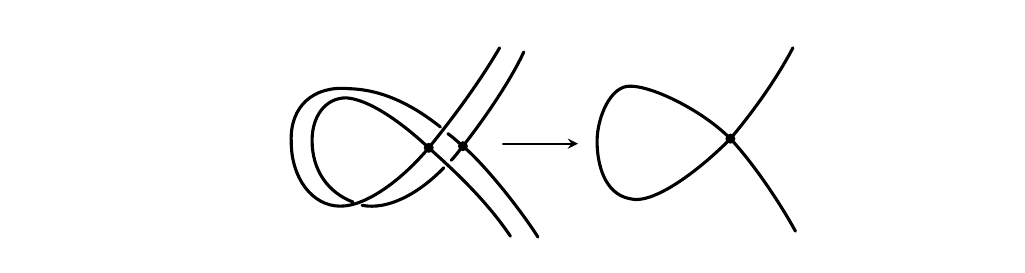
\begin{tikzpicture}[
    x=.3bp, y=-.3bp, line cap=round, line join=round, >=stealth,
    branch/.style={line width=1.12bp}
  ]
  \path[use as bounding box] (-298.3,-10.2) rectangle (865.033,250.133);
  \coordinate (first-node) at (183,134);
  \coordinate (second-node) at (224,132);

  % One component passes behind the other near its upper arc.
  \draw[branch] (268,14)
    .. controls (244,55) and (213,97) .. (first-node)
    .. controls (152,171) and (109,204) .. (77,204)
    .. controls (43,204) and (18,170) .. (18,127)
    .. controls (16,84) and (45,59) .. (87,63)
    .. controls (127,64) and (163,82) .. (197,109);
  \draw[branch] (206,117)
    .. controls (213,122) and (218,127) .. (second-node)
    .. controls (249,153) and (291,205) .. (314,241);

  % The other underpasses lie just below the two crossings.
  \draw[branch] (297,19)
    .. controls (282,52) and (250,99) .. (second-node)
    .. controls (219,138) and (214,145) .. (210,149);
  \draw[branch] (201,158)
    .. controls (171,189) and (134,209) .. (103,203);
  \draw[branch] (92,199)
    .. controls (63,188) and (43,162) .. (43,125)
    .. controls (43,96) and (59,74) .. (84,74)
    .. controls (112,76) and (151,104) .. (first-node)
    .. controls (219,166) and (254,200) .. (281,240);
  \fill (first-node) circle[radius=1.8bp];
  \fill (second-node) circle[radius=1.8bp];

  \draw[->,line width=.61bp] (272,129) -- (362,129);

  \coordinate (node) at (545,123);
  \draw[branch] (620,14)
    .. controls (600,52) and (572,91) .. (node)
    .. controls (517,152) and (455,204) .. (424,195)
    .. controls (394,189) and (385,154) .. (385,126)
    .. controls (385,98) and (401,59) .. (425,60)
    .. controls (451,60) and (510,88) .. (node)
    .. controls (572,152) and (604,199) .. (623,234);
  \fill (node) circle[radius=1.8bp];
\end{tikzpicture}
